\documentclass[12pt]{article}

\usepackage{setspace}
\usepackage{indentfirst}
\usepackage{graphicx}
\usepackage{caption}
\usepackage{url}
\usepackage{framed}
\usepackage[title]{appendix}
\usepackage[hang,flushmargin]{footmisc}

\captionsetup{font=small}
\newcommand{\code}[1]{\texttt{#1}}

\title{Record Locking Methods in the System for Managing Academic Records and Transcripts}
\author{Lucas Kushner}
\date{\today}

\begin{document}

\begin{titlepage}
    \maketitle
    \thispagestyle{empty}
\end{titlepage}

\newpage\null\thispagestyle{empty}\newpage

\pagenumbering{roman}
\doublespace

\section*{Abstract}
\begin{verbatim}
ToDo
- Change all timestamp to lock_time
- Change all recordId to key
- Change all userId to locker
- Acknowledgements
- Update section 3 to reflect the Unified lock table
\end{verbatim}

\newpage

\section*{Acknowledgements}
This is where my acknowledgements will go.

\newpage

\tableofcontents

\newpage
\pagenumbering{arabic}
\section{Introduction}

\subsection{Background}

After a destructive 11-year civil war that ended in 2001, the nation of Sierra Leone remains in the process of rebuilding its governmental and educational infrastructure. The University of Sierra Leone and Njala University, the country's two major universities, play an important role in providing education, supporting research, and producing alumni who will be instrumental in rebuilding their nation. As both universities continue to develop and expand, using accessible academic and administrative records will be a critical component in institutional capacity building. Currently, these institutions maintain their records purely on paper. By managing computerized records, they will be able to further establish and communicate educational requirements, monitor and support students' educational progress, forecast institutional needs, and assess and document progress toward institutional goals.

Although electronic records are a high priority for these universities, currently no free or Open Source project exists which is suitably equipped to meet their needs. To address this issue, we have proposed combining two existing projects, the Record and Activity Management Program (RAMP), and System for Managing Academic Records and Transcripts (SMART) to produce a dynamic and adaptable system for electronic record keeping.

RAMP provides a framework which makes the creation and implementation of dynamic websites much more flexible, by working off of a dynamically defined database structure. In essence, RAMP allows the creation and use of tables and activities within a web application, without explicitly identifying the tables in the code itself. This is instead done by defining the desired structure of data to be used in a series of configuration files. RAMP allows users to view these tables (or a selected set of columns), search for entries based on certain field values, modify, add and delete records, all in a fashion which is designed to be generic and easily adaptable to different database schemas.

SMART was originally a system used by the Registrar's Office at Kalamazoo College for managing academic records and electronic course registration and placement. It consists of a database structure which has been tuned to the needs of an academic institution, with facilities for organizing curriculum records (including courses of study, courses or modules, and individual offerings), instructor records, and student records.

Each of these two projects is meritable in its own right, however by combining the two we hope to create a new kind of record management system that will be fully functional for academic institutions, yet flexible enough to adapt to the different internal structuring of data within any given college or university. Currently, these projects are being combined to create a new SMART system which runs using RAMP as its framework for managing and displaying data. By taking this approach, we can take advantage of the deeply defined database structure utilized in the previous SMART system, while running atop the flexibly stable RAMP system for managing the data. In doing so, we aim to create a free, robust, and dynamic records management and administration infrastructure for these two universities. Ideally, the final product will also be one which could be easily adapted to different schools and systems with minimal changes to code, providing a solution that any variety of universities would be able to implement in the future.

\subsection[Structure of SMART]{Structure of SMART\footnote{From this point onward, the term "SMART" will be used in reference to the newer system which is a combination of the RAMP and SMART systems as described previously.}}

Several of the most popular web technologies are integrated throughout SMART. At the most basic level, SMART operates on top of a combination of an Apache web server, MySQL database, and the PHP server-side scripting language. This is a very common web-development setup typically referred to as AMP. However, on top of these basic tools, the core functionality and implementation of SMART is made possible through the use of a PHP library known as Zend Framework.

Zend is a popular, modular implementation of a Model-View-Controller (MVC) framework used for powering web applications written in PHP. The MVC application development paradigm outlines a flexible yet powerful structure for the creation of complex applications, and so was perfectly suited for the SMART project. The basic principle is concerned with the separation of responsibilities within the program. The Model component is responsible for managing all direct interactions with the data, outlining its structure, and providing the necessary interfaces and functions to interact with it. On the opposite end of the spectrum, the View components are purely responsible for what the user sees from the application, and handling all logic related to the presentation of data. The Controller is the bridge which connects the data and the user interface, defining and mediating interactions between the Model and View. Whenever data is updated in the View, the Model needs to know how to update the database, and contrastingly, when an update is made to the data the View needs to be notified to present the updated data. Managing these interactions is the core function of a Controller. By splitting up responsibilities in this fashion, the MVC framework keeps the structure of a project neatly organized while still fulfilling the requirements of a complex and dynamic application.

\begin{figure}[h]
    \begin{center}
        \centerline{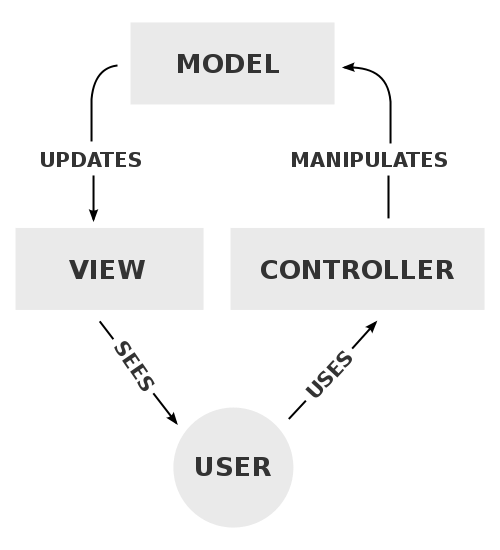
\includegraphics[width=2.1in]{diagrams/MVC.png}}
    \end{center}
    \vspace{-20pt}
    \begin{spacing}{1.0}\caption{A simple diagram of a Model-View-Controller layout\protect\footnotemark}\end{spacing}
\end{figure}

\footnotetext{Image retrieved from \url{http://en.wikipedia.org/wiki/File:MVC-Process.svg}}

Along with the expansive and powerful set of application development tools provided by Zend Framework and the MVC paradigm, the robust flexibility of SMART is possible primarily due to two of its key features: Activities and Tables\footnote{Throughout this paper, we will be using the capitalized word "Table" in reference to Tables that are defined in SMART by Table Settings, whereas the lowercase word "table" will be used in reference to tables in the database.}. 

In SMART, Activities can be thought of as a way for the user to navigate through the program and find the data they are looking for. In essence, an Activity is a webpage which provides a submenu presenting a certain set of Tables that a user can view, gathered under a common heading. However, like much of SMART these Activities are defined not explicitly in code, but in separate configuration files, making them easy to rearrange, modify, and expand. In addition to redirecting users to specific Tables, there are a variety of other Activities that can be used to display information or fire specific actions. For full documentation about Activities, please refer to Appendix A.

Tables are at the heart of SMART's functionality. Without a clean and secure way of accessing and manipulating data, users would not be able to effectively and efficiently achieve their record management goals. In SMART all Tables are defined in configuration files known as Table Settings. These files outline which tables from the database are to be used, which columns should be shown, and specify the labels and formatting of each field. Additionally, Table Settings can outline connections between different database tables, and consolidate data from multiple sources into one Table that is displayed to the user, allowing for the construction of easy-to-use structures that abstract away the underlying complexity of the database. For full documentation about Tables, please refer to Appendix B.

\begin{figure}[h]
    \vspace{10pt}
    \begin{center}
        \centerline{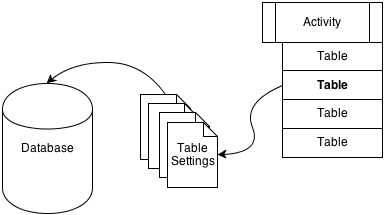
\includegraphics[width=3.5in]{diagrams/SMARTAccess.png}}
    \end{center}
    \begin{spacing}{1.0}\caption{The flow of control in accessing the database in SMART. Activities define a set of tables with which the user can interact. Each Table corresponds to a specific Table Setting file which outlines the relationships to database tables. All definition of database structure is done in the Table Settings, abstracting it away from the program itself.}\end{spacing}
\end{figure}

\subsection{Record Locking}

In a system as expansive and dynamic as SMART many complexities can lead to issues. One such problem that lies at the core of the system is dealing with multiple users attempting to edit data simultaneously, often resulting in an overwrite.The issue of such an overwrite occurs when several users try to access the same piece of data at once. For example, imagine an employee of the registrar is editing the number of students enrolled in a particular course offering. At the same time, another employee also attempts to alter the number of students enrolled, representing a different set of students. With both employees editing the same data, only the last change made will be saved, overwriting the previous change. Such corruption of data could have dire consequences depending on the circumstances.  

One standard solution to deal with this issue is known as “record locking”. Record locking is a way of managing data to assure its integrity, and prevent data from accidentally being overwritten. Several techniques have been developed for “locking” the data, all aiming to prevent multiple users from simultaneously altering it. While a variety of different database and application level implementations exist, the realm of possible solutions operates along two main paradigms: optimistic and pessimistic locking. 

With optimistic locking, multiple users are allowed to continue editing the data simultaneously. The data is only locked when a specific user actually writes their changes to the database. In this situation, whenever a user attempts to write their data, a version number is checked to verify that no new data is present. Only then will the user be notified that a conflict has occurred, at which point they must edit their data again and retry. This method allows several users to continue editing data while still locking the data when it is written. However, the last minute notification of data changes could prove frustrating or confusing to the user.

On the other hand, the pessimistic locking strategy uses what is called a “lock table” to lock specific records, and keep track of who is editing a given record. This table includes the unique ID of the record, the user that is editing it, and the timestamp marking when the user gained access to the record. Whenever a user attempts to edit a record, the lock table is checked to see if the record in question is already being edited. In that case, the user is then immediately notified that a change is in progress, and must wait until that change is submitted before attempting to make their edits. Often, the user will receive a notification once the data has been unlocked, and the page will automatically display the editable data. Although this system is much stricter in its protection of the data, this can lead to an additional problem. In the case known as “deadlock”, two locked processes are waiting for each other to finish before they are able to unlock. Because of this possibility, careful database and software design is necessary when choosing to lock data in a pessimistic fashion.

\newpage
\section{Record Locking in SMART}

\subsection{Challenges and Considerations}

In approaching the issue of record locking, SMART presents an interesting challenge to finding an appropriate implementation. One significant complexity in the problem, is that a “Table” in SMART often consists of data that is pulled from several different tables in the database. For example, when a user attempts to edit the data for a specific course offering, they may see information about the course itself, about the professor of the course, and about the current enrollment. While it makes sense to show all of this information on one page in SMART, the offering's information comes from a Courses table, while the professor and student information comes from a separate Person table. Although the application conveniently abstracts away the underlying database structure, the appropriate entries in both tables must all be locked in order to ensure that all applicable data is protected from overwrites.

Some of these tables, such as the Person and Courses, have a high-frequency usage throughout various Activities in SMART, and therefore strict locking of that data is critical to maintaining its integrity. However, other tables may be accessed much less frequently, and therefore implementing a full-featured record locking system could contribute significant complexity to the structure of data and program execution, with little benefit in terms of realized record management. For example, as student information and course enrollment changes, clearly the Student and Courses tables will be used frequently, and need locking mechanisms in place. However, a Terms table containing information about the start and end of academic terms will likely only be edited once or twice each year, and any mistaken overwrites would be non-detrimental and easily fixed. Therefore, creating a lock table and setting up the locking infrastructure for Terms is too much effort with not enough payback. Thinking this way about which tables to lock is a necessary for the producing an efficient and sensible implementation of record locking throughout SMART.

\subsection{Design of Specific Implementation}

Taking these various factors into account, we decided to implement a strongly pessimistic record locking system. In making this decision there were several considerations that were addressed. Firstly, the information that is most frequently edited in an academic records system generally has a direct relationship to a student or professor's work, and so any mistaken changes to this data could have a significant and stressful impact. Therefore, locking the data in a pessimistic fashion makes the most sense to minimize such mistakes. Additionally, maintaining version numbers on the data, as is done in optimistic locking systems, adds a significant amount of overhead in its implementation and development, and so for the sake of both ease-of-implementation and efficiency, a pessimistic approach was chosen.

In general, pessimistic systems tend to have some sort of mechanism for notifying a locked-out user when the desired resource has become available. While implementing this into SMART is definitely feasible, we have decided not to implement this feature, and instead simply notify a locked-out user to try again later. The reasoning behind this has to do with the working environment of a Registrar's office. Typically, a particular employee may have a long list of updates that need to be made to a certain set of records, involving many different students, faculty, and courses. If they were to run into a record that was locked, they would likely not wait around, and instead continue on to the next item on their list, retrying the locked record later on. With a workflow such as this, it would not be pragmatic to expend resources checking for records to unlock when the majority of the time the user will simply brush over locked data and move on, rendering the checking mechanism unnecessary.

\begin{center}
\begin{figure}[h]
    \centering
    \centerline{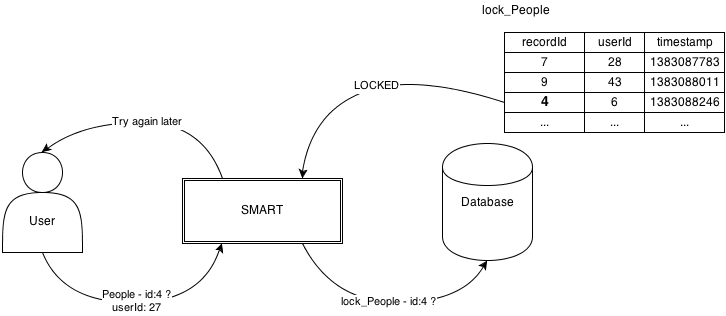
\includegraphics[width=7in]{diagrams/InitialLockDesign.png}}
    \begin{spacing}{1.0}\caption{Design of initially proposed locking system. When the user requests a particular record, the record and user IDs are sent to SMART, which then checks the appropriate lock table and notifies the user if there is a lock. In this model, SMART is programmed with knowledge of the lock table structure in the database.}\end{spacing}
    \vspace{-20pt}
\end{figure}
\end{center}

\subsection{Definition of Locking Relationships}

After coming up with an initial design we set out to begin implementation, and immediately ran into the issue of defining which lock tables in the database would correspond to different Tables in SMART. Originally, our design lent itself to explicitly including logic within the code for determining which lock table corresponded to a certain set of data. However, the power of SMART is that table relationships are not explicitly defined, but instead can be easily configured through the use of Table Settings. To follow this paradigm, it is necessary to define locking relationships in a dynamic fashion, such that SMART could be implemented on any database structure without having to modify the code itself.

One approach would be to define specific locks for each field of a Table in the Table Setting file. This is the approach used by SMART for mapping specific fields that the users sees to the columns of the corresponding database table. The issue arises when considering the possibility of an incorrectly defined Table Setting. Imagine that a user creates a new table setting but neglects to set up the locking mechanisms. If such mechanisms were purely defined by the files, the possibility exists for a user to create a Table without any locking, exposing a significant vulnerability in a fundamental part of the system.

Our solution to this problem is to instead create a new database table which maintains the information about mapping specific data to its appropriate lock table. Currently, SMART assumes the existence of only two specific tables: \code{ramp\_auth\_auths}, and \code{ramp\_auth\_users}. These tables are responsible for logic related to user authentications and permissions, while all other aspects of the application are flexibly defined in Table Setting files. By adding another program-specified table (ie. \code{ramp\_locks}) and using it to manage locking information, we can force specific locking relationships on the database level, as opposed to the settings level. Doing so means that locks are enforced completely regardless of any specific Table Setting, thereby making it impossible for a user to accidentally create unlocked access to the data. The downside to this approach is that it creates more work for the database administrator during the initial setup of the database. However, the extra effort is necessary to ensure a secure and stable record locking mechanism

\begin{center}
\begin{figure}[h]
    \vspace{-10pt}
    \centering
    \centerline{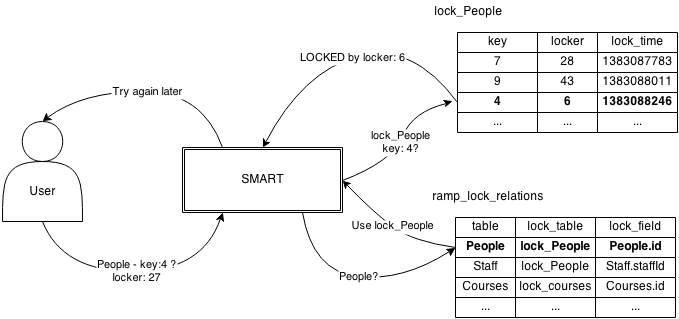
\includegraphics[width=7in]{diagrams/SecondLockDesign.png}}
    \begin{spacing}{1.0}\caption{Flow of control for the updated locking solution in SMART. We see that the program checks the \code{ramp\_locks} table for the defition of locking relatoinships, and uses those values to enforce locking at the database level.}\end{spacing}
    \vspace{-10pt}
\end{figure}
\end{center}

As shown in the figure above, the proposed \code{ramp\_locks} table contains three columns: \code{table}, \code{lock\_table}, and \code{lock\_field}. As one might expect, \code{table} and \code{lock\_table} specify the name of the table in the database and the corresponding \code{lock\_table} which will manage its locks. Beyond these basic record locking components, the \code{lock\_field} column gives this particular locking mechanism enhanced flexibility. Ultimately, the entry in \code{lock\_field} will correspond to the \code{recordId} column of the \code{lock\_table}. Because any column in the table can be used in \code{lock\_field}, this allows for both primary and foreign keys to be used as a locking trigger, which in turn creates the possibility for powerful locking schemes on tables that pull data from multiple sources. In the example shown in the figure, when a user begins editing a particular entry in the Staff table, SMART will use the value of Staff.staffId as the lock in \code{lock\_person}. Because of this, if another user tries to edit the Person with that ID from any other part of SMART, they will be notified that the resource is locked. In this way, record locks are able to be persistent regardless of what particular Activity they originate from. This feature of our record locking system is the critical component in establishing a technique that can handle the requirements of SMART.

\subsection{A Unified Lock Table}
The above management of locking relationships allows locking to be forced on the database level. However, this system still involves many necessary alterations to the database for any particular system, specifically, adding lock tables for each of the appropriate database tables. If at all possible, SMART will operate in such a way that minimal changes are necessary when adapting to a new system. To address this issue, we propose maintaining the same method for defining locking relationships in the \code{ramp\_locks} table, but unifying the lock tables into one required table (ie. \code{ramp\_locks\_locks}), in which all existing locks are stored.

\begin{center}
\begin{figure}[h]
    \centering
    \centerline{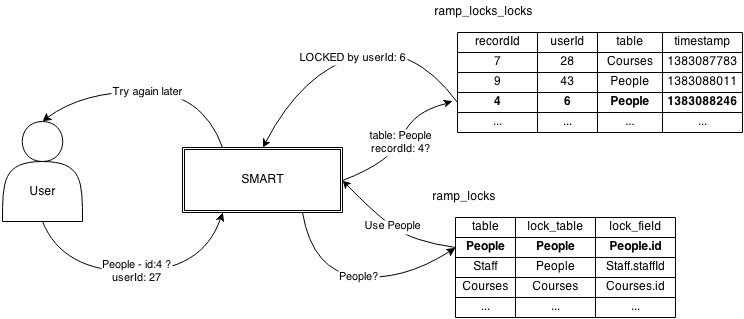
\includegraphics[width=7in]{diagrams/UnifiedLockDesign.png}}
    \begin{spacing}{1.0}\caption{Caption will go here.}\end{spacing}
\end{figure}
\end{center}

This master lock table would need to contain more detailed information than the generic locking table structure discussed previously. For example, since we are using one table to maintain locks for any number of tables, it is necessary to keep track of which table a particular lock belongs to, in addition to its \code{recordId} and \code{userId}. By checking all three of these criteria, it is possible to maintain very specific locks on particular records using only one table, while maintaining the data relationships on which to lock in another table. The end result of such a locking system is shown in the figure below.

\newpage
\section{Alternative Implementations and Solutions}

Throughout this paper, the majority of our exploration of record locking has been specifically attuned to the needs and nature of SMART. However, the development of our implementation and its various features and components involved in-depth analysis of this specific system, and the consideration of a variety of possibilities. Next, we will discuss alternative systems for record locking, including potential features for other pessimistic systems, and optimistic alternatives.

\subsection{Pessimistic Systems}
One such additional feature for a pessimistic system would be a mechanism for notifying a locked-out user when the desired resource has become available, as described previously. Such a notification typically involves an Asynchronous Javascript and XML (AJAX) function call that pings the server at regular intervals to check if the data is still locked. Once the record is unlocked, the user is then redirected to the editing page, which has been populated with the recently updated information. In such a system as this, it is also necessary to implement some form of access queue, to handle the scenario in which several users attempt to access the same page while a record is being edited. This access queue could be implemented relatively easily by performing additional logic when checking a record's availability, as demonstrated in the code fragment below.

\begin{framed}
\begin{spacing}{1.0}
\begin{verbatim}
function checkLock($recordId, $userId)
    // Access queue logic is implemented by ordering 
    // by time and seelcting only the most recent lock
    $lockRow = SELECT * FROM locks
               WHERE recordId=$recordId 
               ORDER BY lock_time ASC LIMIT 1;
    if ($lockRow['userId'] == $userId)
        return true;
    else
        return false;

\end{verbatim}
\end{spacing}
\end{framed}

As opposed to our method of managing lock relationships using a separate \code{ramp\_locks} table in addition to a variety of lock tables, it would be possible for the database to be setup in such a way that every table had its own \code{lock\_table}. In this case, the software would simply need knowledge of which tables were being accessed to immediately know which lock tables to use. For systems where there are numerous tables, many of which contain sensitive and frequently accessed information, a solution such as this may be the most appropriate.

\subsection{Optimistic Systems}
Alternatively, depending on the structure and purpose of the application an optimistic locking system may make more sense. In SMART, the sensitivity of data and workflow of academic records management implied that the use of pessimistic record locking was better suited for the project. Scenarios in which an optimistic solution would be better suited include cases where it is unviable to make all users wait to edit a certain record, or where many unrelated users are accessing data from different locations. A perfect example of this kind of system is a large, wiki type website, such as Wikipedia. In optimistic systems such as these, typically the program must manage version numbers on all edits to records. When a user attempts to write data, the original version number is included with the submitted data and checked against the version number stored in the lock table. If there is a versioning conflict (ie. if another user has submitted new data during the interval that the initial user was editing), the user is then notified and must handle any conflicting data, as demonstrated in the snippet below.

\begin{framed}
\begin{spacing}{1.0}
\begin{verbatim}
function submitData($recordId, $userId, $data)
    $dataRow = SELECT * FROM data_table 
               WHERE recordId=$recordId;
    if ($dataRow['version'] == $data['version'])
        UPDATE data_table
        SET version=$data['version'], ...
        WHERE recordId=$recordId
    else
        // If there was a conflict, send them to a
        // page to sort out conflicting data
        redirectToConflictPage($recordId, $data)

\end{verbatim}
\end{spacing}
\end{framed}

One of the primary advantages present in using an optimistic system as opposed to a pessimistic one is that all users are able to edit data simultaneously, only being locked out at the time of submission. If good systems are implemented for managing conflicts, optimistic systems have the potential to allow for much more efficient editing by many users. However, this method puts more responsibility on the user to make the appropriate decisions when dealing with conflicts and merging data. Furthermore, if the conflicts are significant, than it may not be clear which is correct. While it creates the opportunity for concurrent data modification, optimistic record locking also opens up the possibility of significant frustrations for the end user.

\newpage
\section{Conclusion}

\subsection{Summary}
Throughout this paper, we have explored various potential solutions to the problem of record locking. In the two major paradigms of solutions - pessimistic and optimistic locking - there are a variety of different approaches that may be suited to different kinds of software systems. Additionally, for any given record locking mechanism there are a several features and alterations that can be made to fine-tune the design pattern to a system’s needs, as well as increase the usability and maintainability of whatever locking system is to be implemented.

By considering the merits and disadvantages of both pessimistic and optimistic systems, it was concluded that a strongly pessimistic approach was the most appropriate for meeting the needs of SMART. In addition to the traditional methodology of pessimistic record locking, it was necessary for us to include an additional layer of logic to preserve the dynamically defined table structure that is characteristic to SMART. To address this, we propose defining database locking relations in a required table called \code{ramp\_locks}, thereby enforcing record locking on a database level. While such a system adds additional overhead for an institution setting up SMART, it creates secure locking relationships that can maintain the integrity of data throughout the application.

\subsection{The Future of SMART}

\begin{appendices}
\clearpage
\section{Activity Documentation}
Activities in SMART provide the core navigation of the software, organizing specific tables and tasks in related groups, and giving the user the ability to find and edit the data that they need. They are specified in settings files ending in the .act file extension.

These files consist of an activity list specification, defining the activities to include in the list in the order in which they should appear. The valid types of activities are listed below, along with their required attributes which must also be defined in the file:

\begin{framed}
separator (A horizontal separator)
    -- No properties required
comment (A textual comment to give information about the activity)
    -- comment: The text of the comment to be displayed
setting (“sequence” is a synonym) (Redirects the user to a Table)
    -- title: A short title (should fit into a button)
    -- description: A brief description of the setting referred to
    -- source: The source for the setting (the name of the Table Setting file, without suffix)
report (Generates a specific report using existing data, see Report specifications)
    -- title: A short title (should fit into a button)
    -- description: A brief description of the setting referred to
    -- source: The source for the setting (the name of the Table Setting file, without suffix)
html
    -- html: The html to be rendered
controllerAction (Fires a particular controller action in Zend)
    -- title: A short title (should fit into a button)
    -- description: A brief description of the setting referred to
    -- controller: The controller to use
    -- action: The action to use
    -- parameter: Parameter string using key1=param1\&key2=param2 format
url (Redirects the user to a webpage)
    -- title: A short title (should fit into a button)
    -- description: A brief description of the setting referred to
    -- url: The url address to go to
activityList (Redirects the user to another Activity)
    -- title: A short title (should fit into a button)
    -- description: A brief description of the setting referred to
    -- source: The source for the setting (the name of the Table Setting file, without suffix)
\end{framed}

\clearpage
\section{Table Documentation}

\clearpage
\section{System Specifications}

For development purposes, our backend for the SMART system used a Cross-platform Apache, MySQL and PHP distribution known as XAMPP. This package allows for the easy installation of these various components, as well as providing default configurations for easy use. Additionally, we used Zend Framework 1.12 library for the backbone of the application. Although Zend is currently in version 2, we continued using 1.12 because much of SMART had been written in years prior to the new version, and a variety of significant changes were made to the framework that could not be easily updated within the existing project.

Further investigation is still needed to determine the minimum possible hardware and software system requirements for SMART. Most tests and development discussed in this paper have taken place on a Linux system, with software specifications as outlined below:
\\

\begin{spacing}{1.0}
\noindent\textbf{Machine Specifications} \\
Linux Mint 14 Nadia \\
Intel Core i5 M430 @ 2.27 GHz \\

\noindent\textbf{Development Software} \\
XAMPP for Linux (1.8.1) \\
Apache (2.4.3) \\
MySQL (5.5.27) \\
PHP (5.4.7) \\
phpMyAdmin (3.5.2.2) \\
Zend Framework (1.12.3) \\
VIM - Vi IMproved (7.4)
\end{spacing}


\end{appendices}

\end{document}
